\documentclass[]{elsarticle} %review=doublespace preprint=single 5p=2 column
%%% Begin My package additions %%%%%%%%%%%%%%%%%%%
\usepackage[hyphens]{url}

  \journal{BioR\(\chi\)iv} % Sets Journal name


\usepackage{lineno} % add

\usepackage{graphicx}
%%%%%%%%%%%%%%%% end my additions to header

\usepackage[T1]{fontenc}
\usepackage{lmodern}
\usepackage{amssymb,amsmath}
\usepackage{ifxetex,ifluatex}
\usepackage{fixltx2e} % provides \textsubscript
% use upquote if available, for straight quotes in verbatim environments
\IfFileExists{upquote.sty}{\usepackage{upquote}}{}
\ifnum 0\ifxetex 1\fi\ifluatex 1\fi=0 % if pdftex
  \usepackage[utf8]{inputenc}
\else % if luatex or xelatex
  \usepackage{fontspec}
  \ifxetex
    \usepackage{xltxtra,xunicode}
  \fi
  \defaultfontfeatures{Mapping=tex-text,Scale=MatchLowercase}
  \newcommand{\euro}{€}
\fi
% use microtype if available
\IfFileExists{microtype.sty}{\usepackage{microtype}}{}
\usepackage[margin=1in]{geometry}
\bibliographystyle{elsarticle-harv}
\ifxetex
  \usepackage[setpagesize=false, % page size defined by xetex
              unicode=false, % unicode breaks when used with xetex
              xetex]{hyperref}
\else
  \usepackage[unicode=true]{hyperref}
\fi
\hypersetup{breaklinks=true,
            bookmarks=true,
            pdfauthor={},
            pdftitle={Measurement error associated with gait cycle selection in treadmill running at various speeds},
            colorlinks=false,
            urlcolor=blue,
            linkcolor=magenta,
            pdfborder={0 0 0}}
\urlstyle{same}  % don't use monospace font for urls

\setcounter{secnumdepth}{0}
% Pandoc toggle for numbering sections (defaults to be off)
\setcounter{secnumdepth}{0}


% tightlist command for lists without linebreak
\providecommand{\tightlist}{%
  \setlength{\itemsep}{0pt}\setlength{\parskip}{0pt}}






\begin{document}


\begin{frontmatter}

  \title{Measurement error associated with gait cycle selection in
treadmill running at various speeds}
    \author[Centre for Sport Research]{Aaron S. Fox\corref{1}}
  
    \author[Centre for Sport Research]{Jason Bonacci}
  
    \author[UNSW]{John Warmenhoven}
  
    \author[Centre for Sport Research]{Meghan F. Keast}
  
      \address[Centre for Sport Research]{Centre for Sport Research,
School of Exercise and Nutrition Sciences, Deakin University, Geelong,
Australia}
    \address[UNSW]{School of Engineering and Information Technology,
University of New South Wales, Canberra, Australia}
      \cortext[1]{Corresponding Author: aaron.f@deakin.edu.au}
  
  \begin{abstract}
  TODO: Insert abstract\ldots{}
  \end{abstract}
  
 \end{frontmatter}

\hypertarget{introduction}{%
\section{Introduction}\label{introduction}}

Collecting and analysing biomechanical data is a common method for
understanding relationships between running technique and performance
\textbf{\emph{{[}ADD REFS{]}}} or injury/pain \textbf{\emph{{[}ADD
REFS{]}}}, and evaluating changes in running technique following
training or interventions \textbf{\emph{{[}ADD REFS{]}}}. A common
approach across this form of study is to average data from a number of
gait cycles to compute a given biomechanical measure. Calculating this
`representative mean' is therefore thought to be representative of the
individuals broader running technique. Given the inherent variability in
human movement (\textbf{vanEmmerik2000?}), the number of and how gait
cycles are selected to create this `representative mean' appears an
important choice in accurately quantifying an individuals running gait.
However, the number of gait cycles used in biomechanical studies of
running varies across the literature (\textbf{Oliveira2021?}). Further,
from our groups experience reading such studies --- very rarely (if
ever) has the decision process underpinning how many gait cycles are
used been specifically explained.

~

We can collect a significant number of gait cycles from runners during
laboratory- or clinic-based testing, particularly if a treadmill is
used. Having participants settle into a steady rhythm via an extended
period of running may be advantageous in producing a more habitual
running pattern \textbf{\emph{{[}REF for this???{]}}}. The use of a
significant number of gait cycles becomes a greater issue when analysing
these data. Inflated data cleaning (e.g.~labelling and gap filling
motion capture data) and analysis (e.g.~processing frames via inverse
kinematics) times will occur when processing a running trial that uses
many versus fewer gait cycles. Similarly, the increased data storage
needs (i.e.~larger file sizes) associated with trials including more
gait cycles could introduce difficulties in circumstances where data
storage access is limited. There is subsequently a need to understand
the impact gait cycle selection processes have on biomechanical
measures, to help optimise data collection and analysis practices
without adversely impacting the testing outcomes.

~

Oliveira and Pirscoveanu(\textbf{Oliveira2021?}) recently examined the
typical number of gait cycles used in running biomechanics studies.
Studies used 12 cycles on average per runner to describe running
biomechanics, while Very few (5 out of 56 studies examined) used more
than 10 cycles (\textbf{Oliveira2021?}). Oliveira and
Pirscoveanu(\textbf{Oliveira2021?}) subsequently performed a study
investigating the impact of sample size (i.e.~10 to 40 runners) and the
number of gait cycles (i.e.~5 to 40 steps) used on running measures ---
specifically, foot contact time, loading rate, peak vertical ground
reaction force, peak braking force, running speed, and foot contact
angle. They suggested greater than 10 steps are typically required to
achieve stable biomechanical measures in runners, and collecting at
least 25 steps will increase the likelihood of achieving stability in
the range of biomechanical measures examined (\textbf{Oliveira2021?}).
These findings are, however, specific to overground running and the set
of biomechanical measures analysed. Treadmill running is often used in
research (\textbf{VanHooren2020?}), and it is plausible that treadmill
running may incur a different pattern with respect to the number of gait
cycles needed for analyses. Further, Oliveira and
Pirscoveanu(\textbf{Oliveira2021?}) did not examine lower limb kinematic
variables commonly used in gait biomechanics studies. These kinematic
variables can be presented as both `zero-dimensional' (0D; e.g.~peak
values) and `one-dimensional' (1D; e.g.~time-normalised kinematic
waveform) variables \textbf{\emph{{[}ADD REFS{]}}}. Analyses of these
common kinematic variables in both their 0D and 1D forms may yield
additional details with respect to the number of gait cycles required in
biomechanical research. Lastly, Oliveira and
Pirscoveanu's(\textbf{Oliveira2021?}) analyses were driven by
understanding data stability and statistical significance between two
running conditions (i.e.~`normal' vs.~`silent' running). A different
approach focused on understanding the magnitude of `error' introduced by
analysing different numbers of gait cycles can further our understanding
of how gait cycle selection practices impact biomechanical measures.
Specifically, understanding the potential `error' or variability
introduced by selecting a different number of gait cycles can aid in
interpreting the legitimacy of an effect (i.e.~could small effects be
due to the set of gait cycles selected).

~

We sought to extend our current understanding of how the number of gait
cycles selected for analysis impact lower limb kinematic measures from a
continuous bout of treadmill running. First, we examined the magnitude
of `error' introduced in the representative mean compared to the entire
bout of treadmill running when the number of gait cycle samples is
varied. Second, we examined the potential variation introduced in the
representative mean when sampling a specific number of gait cycles from
different sections of the running bout.

\hypertarget{methods}{%
\section{Methods}\label{methods}}

\hypertarget{dataset}{%
\subsection{Dataset}\label{dataset}}

~

We used the public dataset of treadmill running biomechanics from
Fukuchi et al.(\textbf{Fukuchi2017?}). The specifics of this dataset can
be found in the associated paper (\textbf{Fukuchi2017?}). Briefly, this
dataset contains lower-extremity kinematics and kinetics of 28 regular
runners (27 male, 1 female; age = 34.8 ± 6.7 years; height = 176.0 ± 6.8
cm; mass = 69.6 ± 7.7 kg; running experience = 8.5 ± 7.0 years; running
pace = 4.1 ± 0.4 min/km) (\textbf{Fukuchi2017?}). Running kinematics
were collected using a 12-camera 3D motion capture system (Raptor-4,
Motion Analysis, Santa Rosa, CA, United States) and ground reaction
force (GRF) data via an instrumented dual-belt treadmill (FIT, Bertec,
Columbus, OH, United States) (\textbf{Fukuchi2017?}). Participants ran
on the treadmill at three designated speeds (2.5m·s\textsuperscript{-1},
3.5m·s\textsuperscript{-1} and 4.5m·s\textsuperscript{-1}), during which
a three-minute accommodation period was provided followed by a 30-second
data collection period (\textbf{Fukuchi2017?}).

~

We processed the experimental data from Fukuchi et
al.(\textbf{Fukuchi2017?}) using OpenSim 4.0(\textbf{Delp2007?}).
Segment geometry of the generic musculoskeletal model of the pelvis and
lower limb provided by Lai et al.(\textbf{Lai2017?}) were scaled for
each participant using their static calibration trial, which was also
used as a reference for adjusting marker positions on the model. Lower
limb joint angles were calculated using filtered (10Hz low-pass
4\textsuperscript{th} order Butterworth) marker trajectory data within
inverse kinematics analysis. GRF data were filtered using the same
cut-off frequency and filter. The filtering procedures reflected those
originally performed by Fukuchi et al.(\textbf{Fukuchi2017?}). Foot
strike and toe-off events were determined when the vertical GRF crossed
a 20N threshold, also in line with the original
work(\textbf{Fukuchi2017?}).

\hypertarget{data-analysis}{%
\subsection{Data Analysis}\label{data-analysis}}

~

Kinematic variables common to gait biomechanics studies (i.e.~hip
flexion/extension, hip adduction/abduction, hip internal/external
rotation, knee flexion and ankle plantarflexion/dorsiflexion) were
extracted from the right limb for all participants. Data between
consecutive foot strikes were extracted and time-normalised to 0-100\%
of the gait cycle. The time-normalised one-dimensional (1D) curves were
used in subsequent 1D analyses, while a set of peak variables (hip
flexion, hip adduction, hip internal rotation, knee flexion, ankle
dorsiflexion) were calculated and extracted for the zero-dimensional
(0D) analyses.

~

To examine how the number of gait cycles used impacts a participants
representative kinematic mean, we determined `ground truth' values to
compare to for the 0D and 1D kinematic variables by calculating the mean
from all available gait cycles in the 30-second bout of treadmill
running. This value was thought to be the `most representative' of each
participants average running kinematics, and was not influenced by the
selection of a subset of gait cycles from the running bout. We then
iteratively calculated mean values across the kinematic variables using
a range (\emph{n} = 5 --- 30) of gait cycles from the treadmill running
bout. For each iteration, a random sample of \emph{n} consecutive gait
cycles were extracted from the treadmill running bout and used to
calculate a representative kinematic mean. We then compared this
representative kinematic mean to the `ground truth' value for the
respective variable to determine the `error' that gait cycle number
selection could introduce. For 0D variables, the absolute difference
between the representative mean and `ground truth' was recorded in each
sampling iteration. For 1D variables, the absolute difference between
the representative mean and `ground truth' at each point across the
time-normalised gait cycle were calculated, and the peak difference
recorded. The random sampling process for each \emph{n} of gait cycles
was repeated 1,000 times for each participant at each running speed ---
and the `error' values collated to present descriptive statistics
(i.e.~mean ± standard deviation {[}SD{]}, median, range, inter-quartile
range) for each gait cycle number across the kinematic variables and
running speeds.

~

To examine how sampling gait cycles from different sections of the
running bout impacts a participants representative kinematic mean, we
iteratively calculated representative kinematic means using a range
(\emph{n} = 5 --- 15) of randomly sampled consecutive gait cycles from
different sections of the running bout. A smaller range of gait cycles
was required for this analysis to avoid sharing gait cycles between the
calculated means. For each sampling iteration, we randomly sampled
\emph{n} consecutive gait cycles from two sections of the running bout.
We then compared the calculated representative kinematic means between
the two sampled sections to determine the `error' or variation that
selection of gait cycles from different sections of the running bout
could introduce. For 0D variables, the absolute difference between the
two representative means was recorded in each sampling iteration. For 1D
variables, the absolute difference between the two representative means
was calculated at each point across the time-normalised gait cycle, and
the peak difference recorded. The random sampling process for each
\emph{n} of gait cycles was repeated 1,000 times for each participant at
each running speed --- and the error values collated to present
descriptive statistics (i.e.~mean ± standard deviation {[}SD{]}, median,
range, inter-quartile range) for each gait cycle number across the
kinematic variables and running speeds.

\hypertarget{results}{%
\section{Results}\label{results}}

\hypertarget{how-does-the-number-of-gait-cycles-used-impact-the-representative-kinematic-mean}{%
\subsection{How does the number of gait cycles used impact the
representative kinematic
mean?}\label{how-does-the-number-of-gait-cycles-used-impact-the-representative-kinematic-mean}}

~

The mean, variance and range of the absolute error of the representative
kinematic mean (i.e.~compared to the mean from all gait cycles) for the
peak 0D kinematic variables progressively reduced as the number of gait
cycles used increased (see Figures \ref{fig:groundTruthError_runT25_0D},
\ref{fig:groundTruthError_runT35_0D} and
\ref{fig:groundTruthError_runT45_0D}). In particular, increasing the
number of gait cycles used reduced the range of potential error compared
to the `ground truth' mean. Similar magnitudes of `error' were observed
between the 2.5m·s\textsuperscript{-1} and 3.5m·s\textsuperscript{-1}
speeds across the 0D kinematic variables at comparable gait cycle
numbers --- where the maximum errors were less than 1 degree even when
using a small number of gait cycles. This contrasted to the
4.5m·s\textsuperscript{-1} speed where maximum errors typically exceeded
1-2 degrees, particularly for peak hip and knee joint angles when a
lower number of gait cycles were used. Subsequently, a much higher
number of gait cycles (i.e.~25-30) achieved similar magnitudes of error
to fewer gait cycles (i.e.~\textless{} 10) for running at
4.5m·s\textsuperscript{-1} versus the other two speeds, respectively.
The larger `error' values observed at 4.5m·s\textsuperscript{-1}
appeared to be driven by a bimodal distribution of the error --- whereby
certain sampling iterations within the same biomechanical measure could
produce relatively higher versus lower errors (see Figure
\ref{fig:groundTruthError_runT45_0D}). The exception to this difference
at the higher speed was for peak ankle dorsiflexion, where similarly low
`error' values and ranges (i.e.~\textless{} 0.5 degrees) were observed
across all speeds.

~

\begin{figure}

{\centering \includegraphics[width=1\linewidth]{D:/+GitRepos+/biomech-trial-selection/Analysis/GroundTruthComp/Figures/AbsoluteError_NoGaitCycle_runT25_0D} 

}

\caption{Absolute error in peak kinematic variables (i.e. zero-dimensional [0D]) when running at 2.5m·s$^{-1}$ using a subset of gait cycles versus all gait cycles from the 30-second treadmill bout. Darker points and solid lines equate to the mean ± standard deviation. Horizontal lines within boxes equate to the median value, boxes indicate the 25$^{th}$ to 75$^{th}$ percentile, and dashed whiskers indicate the range. Shaded violins are included to illustrate the distribution of values. FLEX — flexion; EXT — extension; ADD — adduction; ABD — abduction; IR — internal rotation; ER — external rotation; DF — dorsiflexion; PF — plantarflexion.}\label{fig:groundTruthError_runT25_0D}
\end{figure}

\begin{figure}

{\centering \includegraphics[width=1\linewidth]{D:/+GitRepos+/biomech-trial-selection/Analysis/GroundTruthComp/Figures/AbsoluteError_NoGaitCycle_runT35_0D} 

}

\caption{Absolute error in peak kinematic variables (i.e. zero-dimensional [0D]) when running at 3.5m·s$^{-1}$ using a subset of gait cycles versus all gait cycles from the 30-second treadmill bout. Darker points and solid lines equate to the mean ± standard deviation. Horizontal lines within boxes equate to the median value, boxes indicate the 25$^{th}$ to 75$^{th}$ percentile, and dashed whiskers indicate the range. Shaded violins are included to illustrate the distribution of values. FLEX — flexion; EXT — extension; ADD — adduction; ABD — abduction; IR — internal rotation; ER — external rotation; DF — dorsiflexion; PF — plantarflexion.}\label{fig:groundTruthError_runT35_0D}
\end{figure}

\begin{figure}

{\centering \includegraphics[width=1\linewidth]{D:/+GitRepos+/biomech-trial-selection/Analysis/GroundTruthComp/Figures/AbsoluteError_NoGaitCycle_runT45_0D} 

}

\caption{Absolute error in peak kinematic variables (i.e. zero-dimensional [0D]) when running at 4.5m·s$^{-1}$ using a subset of gait cycles versus all gait cycles from the 30-second treadmill bout. Darker points and solid lines equate to the mean ± standard deviation. Horizontal lines within boxes equate to the median value, boxes indicate the 25$^{th}$ to 75$^{th}$ percentile, and dashed whiskers indicate the range. Shaded violins are included to illustrate the distribution of values. FLEX — flexion; EXT — extension; ADD — adduction; ABD — abduction; IR — internal rotation; ER — external rotation; DF — dorsiflexion; PF — plantarflexion.}\label{fig:groundTruthError_runT45_0D}
\end{figure}

We observed near identical characteristics of the mean, variance and
range of the peak absolute error of the representative kinematic mean
(i.e.~compared to the mean from all gait cycles) for the 1D kinematic
variables (see Figures \ref{fig:groundTruthError_runT25_1D},
\ref{fig:groundTruthError_runT35_1D} and
\ref{fig:groundTruthError_runT45_1D}). As with the 0D variables, the
potential `error' reduced as the number of gait cycles increased, and
similarly low magnitudes of `error' (i.e.~\textless{} 1 degree) were
observed between the 2.5m·s\textsuperscript{-1} and
3.5m·s\textsuperscript{-1} speeds across the 1D kinematic variables at
comparable gait cycle numbers. Larger `errors' exceeding 1-2 degrees
with lower gait cycle numbers were present at the
4.5m·s\textsuperscript{-1} speed (with the exception of ankle
dorsi/plantarflexion), with this again appearing to be driven by a more
bimodal distribution of samples (see Figure
\ref{fig:groundTruthError_runT45_1D}).

~

\begin{figure}

{\centering \includegraphics[width=1\linewidth]{D:/+GitRepos+/biomech-trial-selection/Analysis/GroundTruthComp/Figures/AbsoluteError_NoGaitCycle_runT25_1D} 

}

\caption{Peak absolute error in kinematic variables across the gait cycle (i.e. one-dimensional [1D]) when running at 2.5m·s$^{-1}$ using a subset of gait cycles versus all gait cycles from the 30-second treadmill bout. Darker points and solid lines equate to the mean ± standard deviation. Horizontal lines within boxes equate to the median value, boxes indicate the 25$^{th}$ to 75$^{th}$ percentile, and dashed whiskers indicate the range. Shaded violins are included to illustrate the distribution of values. FLEX — flexion; EXT — extension; ADD — adduction; ABD — abduction; IR — internal rotation; ER — external rotation; DF — dorsiflexion; PF — plantarflexion.}\label{fig:groundTruthError_runT25_1D}
\end{figure}

\begin{figure}

{\centering \includegraphics[width=1\linewidth]{D:/+GitRepos+/biomech-trial-selection/Analysis/GroundTruthComp/Figures/AbsoluteError_NoGaitCycle_runT35_1D} 

}

\caption{Peak absolute error in kinematic variables across the gait cycle (i.e. one-dimensional [1D]) when running at 3.5m·s$^{-1}$ using a subset of gait cycles versus all gait cycles from the 30-second treadmill bout. Darker points and solid lines equate to the mean ± standard deviation. Horizontal lines within boxes equate to the median value, boxes indicate the 25$^{th}$ to 75$^{th}$ percentile, and dashed whiskers indicate the range. Shaded violins are included to illustrate the distribution of values. FLEX — flexion; EXT — extension; ADD — adduction; ABD — abduction; IR — internal rotation; ER — external rotation; DF — dorsiflexion; PF — plantarflexion.}\label{fig:groundTruthError_runT35_1D}
\end{figure}

\begin{figure}

{\centering \includegraphics[width=1\linewidth]{D:/+GitRepos+/biomech-trial-selection/Analysis/GroundTruthComp/Figures/AbsoluteError_NoGaitCycle_runT45_1D} 

}

\caption{Peak absolute error in kinematic variables across the gait cycle (i.e. one-dimensional [1D]) when running at 4.5m·s$^{-1}$ using a subset of gait cycles versus all gait cycles from the 30-second treadmill bout. Darker points and solid lines equate to the mean ± standard deviation. Horizontal lines within boxes equate to the median value, boxes indicate the 25$^{th}$ to 75$^{th}$ percentile, and dashed whiskers indicate the range. Shaded violins are included to illustrate the distribution of values. FLEX — flexion; EXT — extension; ADD — adduction; ABD — abduction; IR — internal rotation; ER — external rotation; DF — dorsiflexion; PF — plantarflexion.}\label{fig:groundTruthError_runT45_1D}
\end{figure}

\hypertarget{how-does-the-selection-of-gait-cycles-impact-the-representative-kinematic-mean}{%
\subsection{How does the selection of gait cycles impact the
representative kinematic
mean?}\label{how-does-the-selection-of-gait-cycles-impact-the-representative-kinematic-mean}}

~

The mean, variance and range of the absolute error (or variation) of the
representative kinematic mean (i.e.~compared to the mean from all gait
cycles) for the peak 0D kinematic variables remained relatively
consistent irrespective of the number of gait cycles used (see Figures
\ref{fig:samplesComp_runT25_0D}, \ref{fig:samplesComp_runT35_0D} and
\ref{fig:samplesComp_runT45_0D}). At the 2.5m·s\textsuperscript{-1} and
3.5m·s\textsuperscript{-1} speeds, the variation in peak kinematic
variables depending on where gait cycles were sampled from in the
running bout was always less than 1.5 degrees --- however, certain
kinematic variables had the potential to produce larger variation than
others (e.g.~peak knee flexion vs.~peak ankle dorsiflexion) (see Figures
\ref{fig:samplesComp_runT25_0D} and \ref{fig:samplesComp_runT35_0D}).
While the potential variation between gait cycle samples was consistent
with increasing gait cycle numbers at the 4.5m·s\textsuperscript{-1}
speed, a higher average and range of potential variation (i.e.~up to 2-4
degrees) appeared evident across the peak kinematic variables (with the
exception of peak ankle dorsiflexion). As in the previous analysis, we
observed a bimodal distribution of the samples at the
4.5m·s\textsuperscript{-1} speed (see Figure
\ref{fig:samplesComp_runT45_0D}).

~

\begin{figure}

{\centering \includegraphics[width=1\linewidth]{D:/+GitRepos+/biomech-trial-selection/Analysis/SamplesComp/Figures/AbsoluteError_NoGaitCycle_runT25_0D} 

}

\caption{Absolute error in peak kinematic variables (i.e. zero-dimensional [0D]) when running at 2.5m·s$^{-1}$ using a two comparative subsets of gait cycles from the 30-second treadmill bout. Darker points and solid lines equate to the mean ± standard deviation. Horizontal lines within boxes equate to the median value, boxes indicate the 25$^{th}$ to 75$^{th}$ percentile, and dashed whiskers indicate the range. Shaded violins are included to illustrate the distribution of values. FLEX — flexion; EXT — extension; ADD — adduction; ABD — abduction; IR — internal rotation; ER — external rotation; DF — dorsiflexion; PF — plantarflexion.}\label{fig:samplesComp_runT25_0D}
\end{figure}

\begin{figure}

{\centering \includegraphics[width=1\linewidth]{D:/+GitRepos+/biomech-trial-selection/Analysis/SamplesComp/Figures/AbsoluteError_NoGaitCycle_runT35_0D} 

}

\caption{Absolute error in peak kinematic variables (i.e. zero-dimensional [0D]) when running at 3.5m·s$^{-1}$ using a two comparative subsets of gait cycles from the 30-second treadmill bout. Darker points and solid lines equate to the mean ± standard deviation. Horizontal lines within boxes equate to the median value, boxes indicate the 25$^{th}$ to 75$^{th}$ percentile, and dashed whiskers indicate the range. Shaded violins are included to illustrate the distribution of values. FLEX — flexion; EXT — extension; ADD — adduction; ABD — abduction; IR — internal rotation; ER — external rotation; DF — dorsiflexion; PF — plantarflexion.}\label{fig:samplesComp_runT35_0D}
\end{figure}

\begin{figure}

{\centering \includegraphics[width=1\linewidth]{D:/+GitRepos+/biomech-trial-selection/Analysis/SamplesComp/Figures/AbsoluteError_NoGaitCycle_runT45_0D} 

}

\caption{Absolute error in peak kinematic variables (i.e. zero-dimensional [0D]) when running at 4.5m·s$^{-1}$ using a two comparative subsets of gait cycles from the 30-second treadmill bout. Darker points and solid lines equate to the mean ± standard deviation. Horizontal lines within boxes equate to the median value, boxes indicate the 25$^{th}$ to 75$^{th}$ percentile, and dashed whiskers indicate the range. Shaded violins are included to illustrate the distribution of values. FLEX — flexion; EXT — extension; ADD — adduction; ABD — abduction; IR — internal rotation; ER — external rotation; DF — dorsiflexion; PF — plantarflexion.}\label{fig:samplesComp_runT45_0D}
\end{figure}

We observed similar characteristics for the mean, variance and range of
the absolute error (or variation) of the representative kinematic mean
(i.e.~compared to the mean from all gait cycles) for the 1D kinematic
variables when sampling gait cycles from different sections of the
treadmill bout (see Figures \ref{fig:samplesComp_runT25_1D},
\ref{fig:samplesComp_runT35_1D} and \ref{fig:samplesComp_runT45_1D}).
The potential variation remained low (i.e.~\textless{} 1.5 degrees) and
consistent across the different number of gait cycles at the
2.5m·s\textsuperscript{-1} and 3.5m·s\textsuperscript{-1} speeds (see
Figures \ref{fig:samplesComp_runT25_1D} and
\ref{fig:samplesComp_runT35_1D}), whereas the potential variation
remained consistent but increased (i.e.~up to 2-4 degrees), and shifted
to a bimodal distribution at the 4.5m·s\textsuperscript{-1} speed (see
Figure \ref{fig:samplesComp_runT45_1D}). In contrast to the 0D
variables, this shift was evident in all 1D kinematic variables
(including ankle dorsi/plantarflexion).

\begin{figure}

{\centering \includegraphics[width=1\linewidth]{D:/+GitRepos+/biomech-trial-selection/Analysis/SamplesComp/Figures/AbsoluteError_NoGaitCycle_runT25_1D} 

}

\caption{Peak absolute error in kinematic variables across the gait cycle (i.e. one-dimensional [1D]) when running at 2.5m·s$^{-1}$ using two comparative subsets of gait cycles from the 30-second treadmill bout. Darker points and solid lines equate to the mean ± standard deviation. Horizontal lines within boxes equate to the median value, boxes indicate the 25$^{th}$ to 75$^{th}$ percentile, and dashed whiskers indicate the range. Shaded violins are included to illustrate the distribution of values. FLEX — flexion; EXT — extension; ADD — adduction; ABD — abduction; IR — internal rotation; ER — external rotation; DF — dorsiflexion; PF — plantarflexion.}\label{fig:samplesComp_runT25_1D}
\end{figure}

\begin{figure}

{\centering \includegraphics[width=1\linewidth]{D:/+GitRepos+/biomech-trial-selection/Analysis/SamplesComp/Figures/AbsoluteError_NoGaitCycle_runT35_1D} 

}

\caption{Peak absolute error in kinematic variables across the gait cycle (i.e. one-dimensional [1D]) when running at 3.5m·s$^{-1}$ using two comparative subsets of gait cycles from the 30-second treadmill bout. Darker points and solid lines equate to the mean ± standard deviation. Horizontal lines within boxes equate to the median value, boxes indicate the 25$^{th}$ to 75$^{th}$ percentile, and dashed whiskers indicate the range. Shaded violins are included to illustrate the distribution of values. FLEX — flexion; EXT — extension; ADD — adduction; ABD — abduction; IR — internal rotation; ER — external rotation; DF — dorsiflexion; PF — plantarflexion.}\label{fig:samplesComp_runT35_1D}
\end{figure}

\begin{figure}

{\centering \includegraphics[width=1\linewidth]{D:/+GitRepos+/biomech-trial-selection/Analysis/SamplesComp/Figures/AbsoluteError_NoGaitCycle_runT45_1D} 

}

\caption{Peak absolute error in kinematic variables across the gait cycle (i.e. one-dimensional [1D]) when running at 4.5m·s$^{-1}$ using two comparative subsets of gait cycles from the 30-second treadmill bout. Darker points and solid lines equate to the mean ± standard deviation. Horizontal lines within boxes equate to the median value, boxes indicate the 25$^{th}$ to 75$^{th}$ percentile, and dashed whiskers indicate the range. Shaded violins are included to illustrate the distribution of values. FLEX — flexion; EXT — extension; ADD — adduction; ABD — abduction; IR — internal rotation; ER — external rotation; DF — dorsiflexion; PF — plantarflexion.}\label{fig:samplesComp_runT45_1D}
\end{figure}

\hypertarget{discussion}{%
\section{Discussion}\label{discussion}}

A common approach in biomechanical studies of running is to use a subset
of gait cycles from a bout of running, and average across these cycles
to calculate a representative mean for each participant. There is very
little objective analysis or understanding of what underpins the number
and selection of gait cycles used, and the impact this can have on the
error or variation in biomechanical measures. We aimed to understand how
the number of gait cycles selected, and where these are selected from,
during a continuous bout of treadmill running impact the magnitude of
`error' and variation in lower limb kinematic measures. We found that
including a greater number of gait cycles in the calculation of a
representative kinematic mean has the potential to reduce the magnitude
and range of potential `error' in kinematic measures. The potential
error using a reduced number of gait cycles (i.e.~\emph{n} = 5-10) was
relatively small (i.e.~typically \textless{} 1 degree) when running at
2.5m·s\textsuperscript{-1} and 3.5m·s\textsuperscript{-1}, but slightly
inflated (i.e.~1-4 degrees) as running speed increased to
4.5m·s\textsuperscript{-1}. We found similarly small magnitudes and
patterns of variation in representative kinematic means across the
different running speeds when selecting gait cycles from different
sections of the running bout, and these remained relatively consistent
irrespective of the number of gait cycles used.

~

We found that the `error' between the representative kinematic means and
the associated `ground truth' values progressively reduced with an
increasing number of gait cycles. Using a greater number of gait cycles
equated to using a higher proportion of data that were used to create
the `ground truth' --- hence this result is not surprising. More
noteworthy is the scale of `error' when using a reduced number of gait
cycles (i.e.~\emph{n} = 5-10) and the diminishing effect using a larger
number of gait cycles (i.e.~\emph{n} \textgreater{} 15) had. We
typically observed that the maximum `error' or variation with respect to
the `ground truth' was less than one degree even at the lowest number of
gait cycles used with running at the 2.5m·s\textsuperscript{-1} and
3.5m·s\textsuperscript{-1} speeds, but this could increase up to three
degrees at the faster 4.5m·s\textsuperscript{-1} speed. Reducing the
potential variation of `error' compared to the ground truth appeared to
be the main effect of increasing the number of gait cycles used.
However, this typically plateaued and a diminished benefit observed when
using above 15-20 gait cycles. These patterns were consistent across
both the 0D and 1D kinematic approaches. The notion of diminishing
returns above 15-20 gait cycles contrasts with the findings of Oliveira
and Pirscoveanu(\textbf{Oliveira2021?}) --- whereby data stability was
not achieved in the majority of runners using this number of gait
cycles. A clear difference between our study and this existing
work(\textbf{Oliveira2021?}) was the biomechanical measures analysed
(i.e.~joint kinematics vs.~mostly kinetic variables).
Forrester(\textbf{Forrester2015?}) performed a series of simulations
using a similar sequential analysis technique to Oliveira and
Pirscoveanu(\textbf{Oliveira2021?}) to determine the number of trials
required for biomechanical measures with typical means and standard
deviations. This work(\textbf{Forrester2015?}) proposed that nine (± 8)
trials were required to achieve stability of the mean, which is more in
line with our findings of diminishing returns in `error' at 15-20 gait
cycles. The mean and variation of the biomechanical measure being
examined likely plays a significant role in the potential `error' when
using a reduced number of trials (or gait cycles). We saw the largest
potential `errors' in hip and knee flexion when using a smaller number
of gait cycles --- and this is perhaps not surprising given these
measures had the largest means and standard deviations within the
dataset used(\textbf{Fukuchi2017?}).

~

Despite the potential for diminishing returns, our data suggests that
researchers can minimise the potential `error' in representative
kinematic means by using more gait cycles. A simplistic recommendation
from our analyses would therefore be to use as many gait cycles as
possible within such calculations. This does, however, ignore the
practical considerations of storing, cleaning and processing larger
biomechanical data files. If there are no limitations to using a large
number of gait cycles (i.e.~20-30) then this will minimise potential
`error' or variation in calculations. Certain circumstances, such as a
large participant sample or timely computational measures, may
subsequently make using 20+ gait cycles per sample impractical. Our
recommendation is therefore to balance the practical considerations
against the potential `error' or variation in the data that can be
tolerated. Most of the time this will come down to the accuracy of the
measure, or size of the effect researchers or clinicians are interested
in measuring. For example, based on our analyses --- using less than ten
gait cycles to explore a small effect (i.e.~\textless{} 1-2 degrees) in
1D hip or knee flexion continua may be unwise, as the potential
variation in the calculated means could exceed the magnitude of the
effect of interest. Our data suggests as a general recommendation ---
the smaller the expected effect or magnitude of effect of interest, the
greater number of gait cycles should be used for analyses.

~

We observed relatively small variations (i.e.~\textless{} 1.5 degrees)
between representative kinematic means calculated from gait cycle
samples extracted from different sections of the
2.5m·s\textsuperscript{-1} and 3.5m·s\textsuperscript{-1} running bouts,
while these slightly increased (i.e.~2-4 degrees) when examining the
4.5m·s\textsuperscript{-1} speed. This magnitude of variation did remain
consistent irrespective of the total number of gait cycles used. These
findings suggest that once the number of gait cycles used for analysis
is selected --- the decision of where these are selected from will
introduce a small, but consistent amount of variation. The inherent
variability in human movement(\textbf{vanEmmerik2000?}) is the likely
and potentially unavoidable cause of this variation. We randomly sampled
differing sections of the running bout as part of our analyses, and
at-times this generated near zero variation between the two
representative means. Without further inspection of our data we cannot
confirm what generated the reduced variation, but we hypothesise that
the samples with minimal to no variation likely stemmed from using
sections of the running bout in close proximity to one another. We also
cannot determine which section of the running bout is more
representative or `accurate,' as we only compared between samples and
did not extend this comparison to the `ground truth' values. Our data
can only be used to infer the potential magnitude of variation one can
expect when using gait cycles from different sections of the running
bout. The magnitude of this variation once again appears to be driven by
the scale of the mean and standard deviation of the measure
(i.e.~kinematic measures with higher means and standard deviations incur
a greater magnitude of variation). Much like the earlier point raised,
the practical implications of these findings relate to the confidence we
can have in our accuracy of measuring an effect on lower limb kinematics
during treadmill running. If our observed effect does not exceed the
typical variation seen when sampling from different sections of the
running bout, there is a possibility that the observed effect is simply
noise due to the gait cycles sampled. Researchers and clinicians must
therefore be wary of this, particularly when interpreting very small
effects.

~

A point of difference across our analyses was the impact of speed on
inducing greater `error' relative to the `ground truth' and between
representative means from different sections of the gait bout.
Specifically, the 4.5m·s\textsuperscript{-1} trials induced higher
values in these metrics relative to the 2.5m·s\textsuperscript{-1} and
3.5m·s\textsuperscript{-1} trials. There are various potential reasons
for why we observed these results. Faster running speeds induce larger
means and standard deviations across kinematic
variables(\textbf{Fukuchi2017?})\textbf{\emph{{[}OTHER REFS?{]}}},
particularly in those we observed a more dramatic increase in `error'
for at 4.5m·s\textsuperscript{-1} (i.e.~hip and knee flexion). Much like
our theory when comparing `error' between different kinematic variables,
we propose that the larger means and standard deviations at higher
speeds introduce a greater magnitude of variation across gait cycles ---
and hence greater potential for `error' when sampling from different
gait cycles. Similar kinematic differences are typical between all of
running speeds we examined(\textbf{Fukuchi2017?})\textbf{\emph{{[}OTHER
REFS?{]}}}. It is therefore surprising that the increase in `error' or
variation was not consistent, and most evident and prominent only when
examining the 4.5m·s\textsuperscript{-1} speed. This suggests other
factors may contribute to the increase in `error' we observed. Within
the dataset we examined, participants ran for a three minute
accommodation period at each speed, following which data were collected
over a 30 second period(\textbf{Fukuchi2017?}). The order of running
conditions (i.e.~2.5m·s\textsuperscript{-1}, 3.5m·s\textsuperscript{-1},
4.5m·s\textsuperscript{-1}) was kept consistent for each
participant(\textbf{Fukuchi2017?}). It is possible that these
experimental procedures (i.e.~running at the fastest speed towards the
end of the running period) could have introduced some form of fatigue in
the 4.5m·s\textsuperscript{-1} speed bout. Running in a fatigued state
can increase biomechanical variability \textbf{\emph{{[}ADD REFS{]}}},
while also altering running kinematics compared to a non-fatigued state
\textbf{\emph{{[}ADD REFS{]}}}. If fatigue was present during the final
bout of running, it could theoretically have induced an increase in
kinematic variability during the 30 second period of data collection.
Alternatively, fatigue may have begun to set in within the final 30
seconds of the run --- potentially inducing a change in running
kinematics within the period where data were collected. This latter
explanation may explain the bimodal distribution in `error' we observed
in the 4.5m·s\textsuperscript{-1} running bout, whereby larger `errors'
may have been observed when sampling gait cycles from earlier versus
later sections of the 30 second data collection period. Given we did not
explicitly record the sections where gait cycles were sampled from, this
notion is purely speculative. It should also be noted that the studies
identifying changes in running biomechanics with
fatigue\textbf{\emph{{[}ADD REFS{]}}} used exercise protocols of higher
intensity and longer duration than what participants experienced with
the dataset used in our study. Despite the lack of understanding around
the potential mechanism --- our study demonstrates a greater need to
consider gait cycle sampling practices with running at faster speeds,
and potentially when fatigue is present.

\textbf{FATIGUE STUDIES - `Impacts and kinematic adjustments during an
exhaustive run' // `Effect of fatigue on leg kinematics and impact
acceleration in long distance running' // `Effect of fatigue and gender
on kinematics and ground reaction forces variables in recreational
runners'}

~

Although we identified the potential for measurement `error' or
variation to present based on gait cycle selection --- these were
comparatively small relative to other noted sources of error across the
biomechanical literature(\textbf{Ceseracciu2014?}). The magnitude of
`error' in the present study is eclipsed by the errors or variation
introduced by soft-tissue artefact associated with skin-mounted
markers(\textbf{DIsidoro2020?}), different joint coordinate
systems(\textbf{Sauret2016?}) or gait models(\textbf{Mentiplay2018?}),
kinematic algorithm choice(\textbf{Kainz2016?}), individual testing
experience(\textbf{Sinclair2014?}), or different measurement systems
(i.e.~marker vs.~marker-less)(\textbf{Ceseracciu2014?}).
\textbf{\emph{{[}SOMETHING NEEDS TO BE ADDED HERE TO WRAP THIS
UP\ldots?{]}}}

~

Our results must be considered with respect to the limitations in our
approach. We only examined conditions where \emph{n} consecutive gait
cycles were sampled from a continuous bout of treadmill running at three
set speeds. Different results might be expected with non-consecutive
selection of samples from the running bout, or under different running
conditions (e.g.~outdoor overground running and slower or faster
speeds). Similarly, we focused on peak and 1D waveform data of lower
limb kinematic variables. Other variables used in gait analysis
(e.g.~joint moments, estimates of muscle activation and forces) may
incur variable magnitudes of `error' or variation with respect to gait
cycle selection. Our findings are therefore most applicable to
situations where the analyses and running conditions replicate those of
our experiment. We also inferred `error' via comparison to values
calculated from all gait cycles in an individuals running bout (i.e.~our
`ground truth' value). Although we deemed this the best approach within
our study, it is important to acknowledge that these values may still
not represent the individuals exact or true running kinematics.

\hypertarget{conclusions}{%
\section{Conclusions}\label{conclusions}}

We identified the range of potential `error' or variation in lower limb
kinematics associated with selecting different gait cycles from a bout
of continuous treadmill running. Our findings suggest that selecting as
many gait cycles as possible from the running bout will minimise `error'
--- however, analysing a smaller sample (i.e.~5-10 gait cycles) will
typically result in `errors' or variation less than 3 degrees. Larger
potential `errors' or variation can likely be expected when analysing
kinematic variables with larger means and standard deviations, and
during running at faster speeds. Researchers and clinicians should
consider the balance between the benefits of collecting, processing and
analysing a greater number of gait cycles against the potential
reductions in `error' when determining their methodological approach.
Irrespective of the number of gait cycles used, we recommend that the
potential `error' or variation introduced by this choice be considered
when interpreting effects from treadmill-based running studies (i.e.~is
the magnitude of potential `error' larger than the identified effects
between groups or following an intervention).

\hypertarget{references}{%
\section{References}\label{references}}

\textbf{\emph{{[}TODO: add citation library{]}}}


\end{document}
